
%(BEGIN_QUESTION)
% Copyright 2011, Tony R. Kuphaldt, released under the Creative Commons Attribution License (v 1.0)
% This means you may do almost anything with this work of mine, so long as you give me proper credit

An Allen-Bradley Logix5000 PLC is used to control the starting and stopping of an air compressor based on momentary-contact pushbutton switch inputs as well as high and low pressure switches (PSH and PSL, respectively).  Analyze this program and explain how it is supposed to work:

$$\includegraphics[width=15.5cm]{i02346x01.eps}$$

\filbreak

$$\includegraphics[width=15.5cm]{i02346x02.eps}$$

In particular, answer these following questions:

\begin{itemize}
\item{} Determine the ``normal'' electrical statuses of all switches (e.g. NO or NC) connected to the inputs of this PLC, based on an examination of the respective contact instructions within the PLC program.
\item{} Why is is important that a {\it retentive} timer instruction be used for the calculation of total run-time? 
\item{} What is the significance of the maintenance warning light controlled by this PLC?
\end{itemize}

\vskip 20pt \vbox{\hrule \hbox{\strut \vrule{} {\bf Suggestions for Socratic discussion} \vrule} \hrule}

\begin{itemize}
\item{} Note how all instructions in this Logix5000 PLC program are addressed by {\it tagname} rather than by hardware addresses (e.g. {\tt I:2/6}, {\tt O:3/1}).  How do you suppose the PLC ``knows'' which real I/O points to associate with which instructions in the program?
\item{} How will this system behave if the reset switch fails shorted?
\item{} How will this system behave if the high-pressure switch fails open?
\item{} How will this system behave if the high-pressure switch fails shorted?
\item{} How will this system behave if the low-pressure switch fails open?
\item{} How will this system behave if the low-pressure switch fails shorted?
\end{itemize}

\underbar{file i02346}
%(END_QUESTION)





%(BEGIN_ANSWER)

Input switch electrical ``normal'' statuses:

\begin{itemize}
\item{} {\bf Start} = NO
\item{} {\bf Stop} = NC
\item{} {\bf PSL} = NC
\item{} {\bf PSH} = NC
\item{} {\bf Reset} = NO
\end{itemize}

%(END_ANSWER)





%(BEGIN_NOTES)

The RTO timer instruction is configured to reach its end-count every hour of compressor run time.  It self-resets, with the counter instruction keeping tabs on how many timer cycles (how many hours) the compressor has run.  It is important that an RTO timer instruction is used, so that it will continue to accumulate time even if the compressor runs for less than an hour.

\vskip 10pt

The maintenance warning light turns on when the accumulated run time equals or exceeds 250 hours.

%INDEX% PLC, ladder logic program analysis and explanation

%(END_NOTES)


